\section{EXPERIMENTAL RESULTS}
In this section, we show the experimental results to verify the proposed power budgeting method and analyze its energy efficiency and performance. All data are collected on a PC with Intel I5 2400 CPU and 4 GB memory. Multi-core systems with core number ranging from $9$ to $100$ are used in the experiment, and each core with different dark silicon ratio are tested. The thermal models of these multi-core systems are extracted from HotSpot with default package and chip parameters. The ambient temperature are set to be \SI{20}{\degreeCelsius} for all test cases, and the temperature constraint is \SI{95}{\degreeCelsius}.

\subsection{Effectiveness and energy efficiency test for steady state cases}
In order to test the effectiveness and performance of the new method, we first test it
using a system with small core number ($9$ cores) and show its steady state
behavior step in step. Please note that we show steps of the $9$-core system
because it is easier for the readers to verify the correctness of GDP using
a system with small core number.

Now we demonstrate how our method decides which cores to be active in a
greedy manner for $4$ active cores. For step one, our method looks for the first
active core position. This step is pretty easy even for human, as we
can readily pick the center core, because its position has the best
heat dissipation capability. GDP, unlike human who uses instinct and
experience, picks the core with the largest inner product $\langle
a_j, T_{th}\rangle$, which is exactly the center core. 
Then, our method computes the power
budget for such one active core case. We plot the steady state temperature
distribution caused by the computed power budget in
Fig.~\ref{fig:order_of_cores_1}. As expected, the only active core at
the center has a temperature of \SI{48}{\degreeCelsius}, which is just
the computed optimal temperature for it. Next, our method searches for the
second active core position with the first active core position
fixed. Although all four cores at the corners can be chosen due to
symmetry, the lower left one is picked simply because computer prefers
the first. The updated power budget also leads to
$T_{opt}$ for the two active cores shown in Fig.~\ref{fig:order_of_cores_2}, as expected. For the
third and fourth active cores, GDP locates their positions to be 
upper right corner and lower right corner, with power budget
resulted temperature distributions shown in
Fig.~\ref{fig:order_of_cores_3} and Fig.~\ref{fig:order_of_cores_4},


\begin{figure}
  \centering
  \subfigure[The first step with position and power budget of the first active core determined.]{
    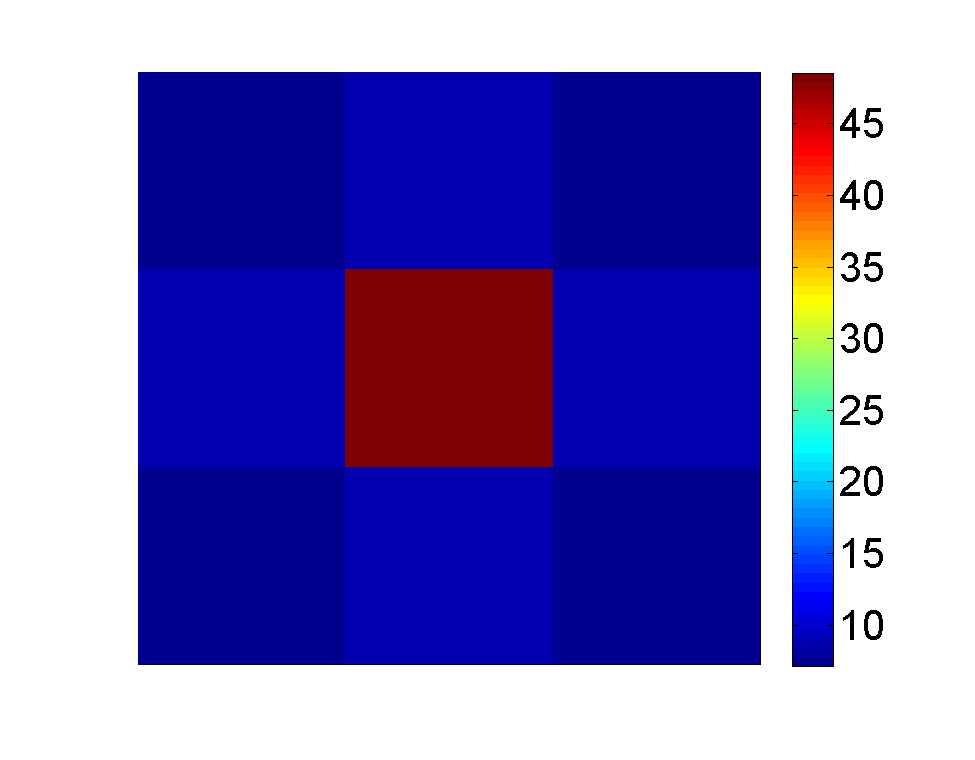
\includegraphics[width=0.46\columnwidth]{fig/order_of_cores_1.eps}\label{fig:order_of_cores_1}
  }
  \subfigure[The second step with positions and power budgets of 2 active cores determined.]{
    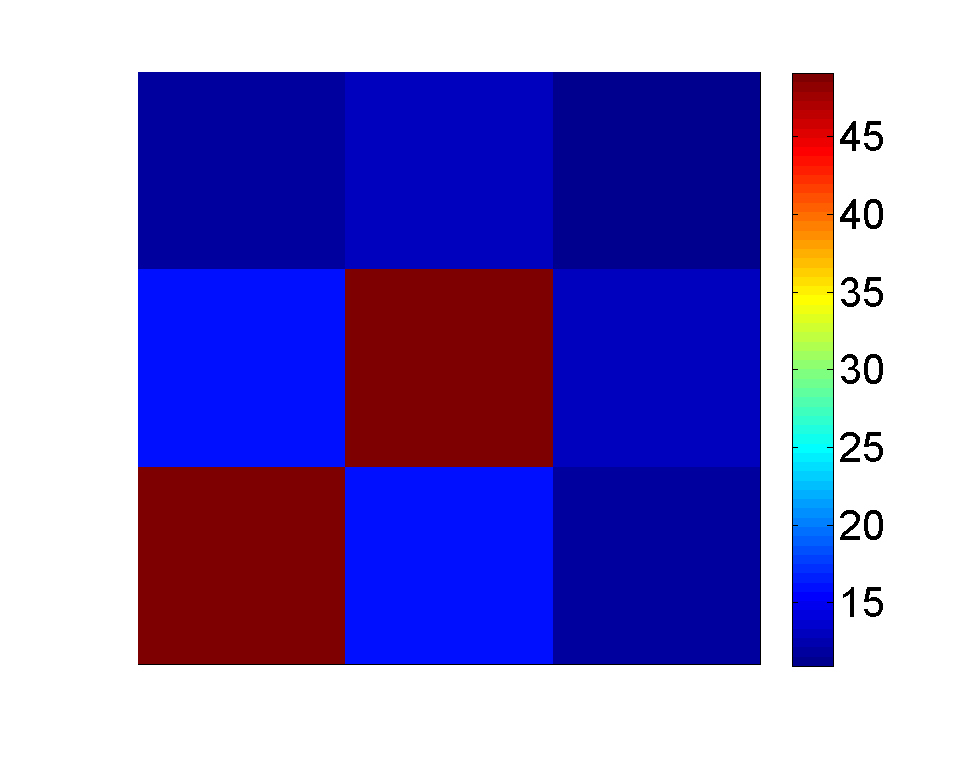
\includegraphics[width=0.46\columnwidth]{fig/order_of_cores_2.eps}\label{fig:order_of_cores_2}
  }
  \subfigure[The third step with positions and power budgets of 3 active cores determined.]{
    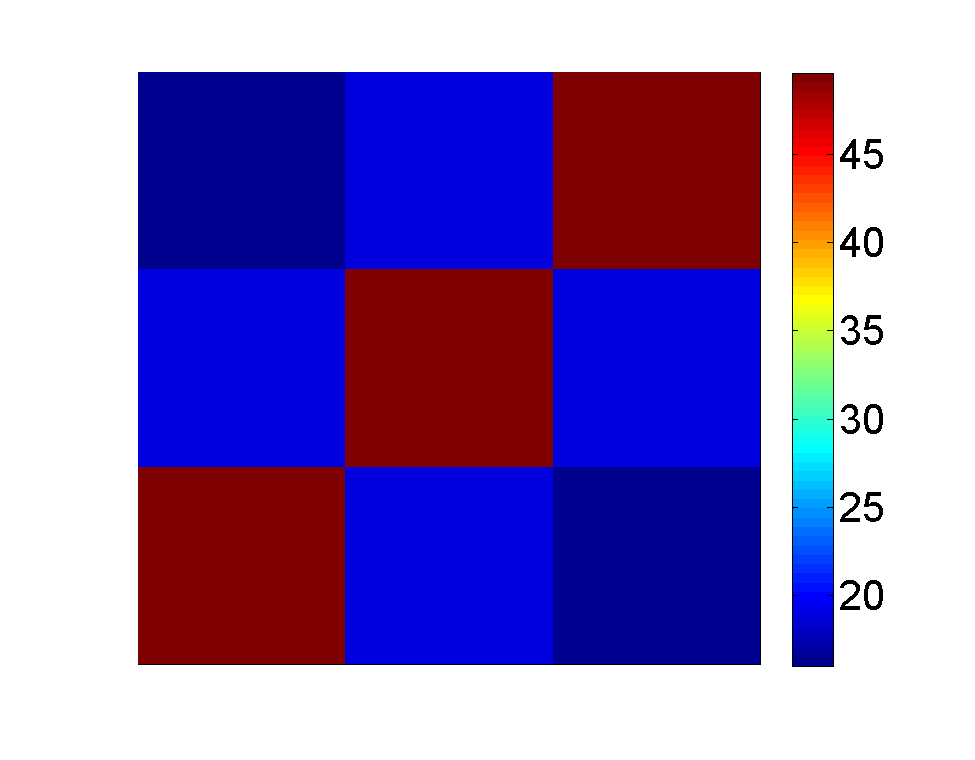
\includegraphics[width=0.46\columnwidth]{fig/order_of_cores_3.eps}\label{fig:order_of_cores_3}
  }
  \subfigure[The fourth step with positions and power budgets of 4 active cores determined.]{
    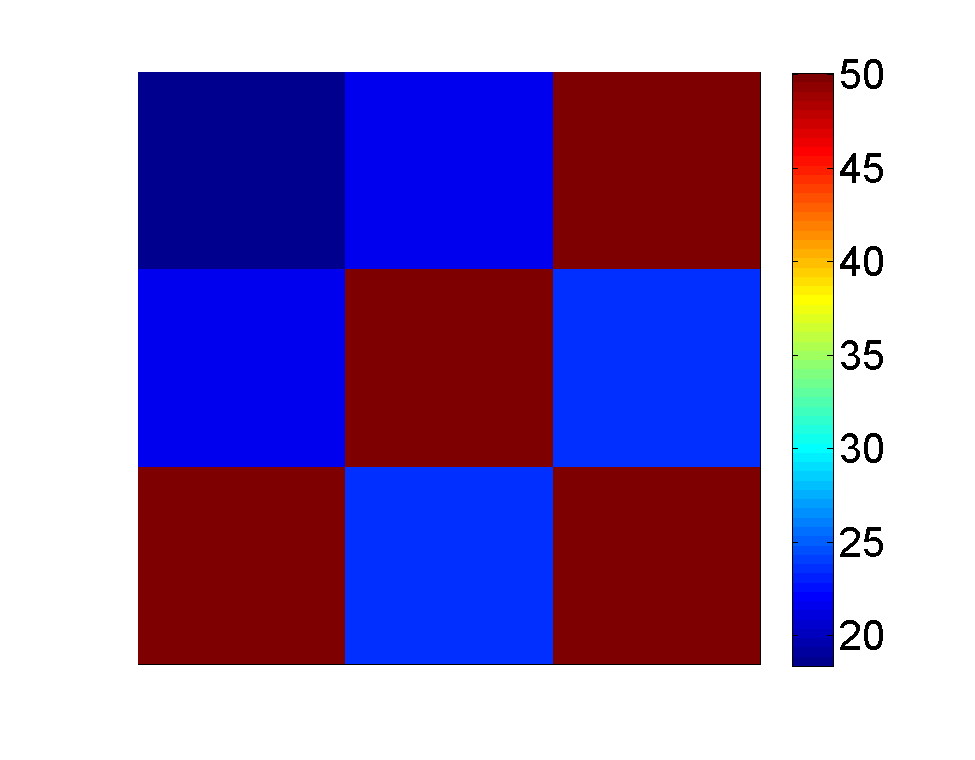
\includegraphics[width=0.46\columnwidth]{fig/order_of_cores_4.eps}\label{fig:order_of_cores_4}
    }
  \caption{Temperature distributions of the 9-core system with the power budget given by our method's first four greedy steps.}
  \label{fig:order_of_cores}
\end{figure}

\begin{table}
%  \color{red}
  \caption{Energy efficiency (in MIPS/Watt) results comparison of steady state power budgeting. "New" stands for our new power budgeting method, "Monte Carlo" denotes the optimal result with maximum PPW from $1000$ Monte-Carlo simulation with varables being active core distribution and DVFS stage of each active core.}
  \label{tab:PPW_steady}
  \centering
  \begin{tabular}{c|c||c|c}
    \hline
    Core & Active     & \multirow {2}{*}{New} &
                                                    \multirow {2}{*}{Monte-Carlo }\\

\#       &   \#       & &   \\
%\#      &   \#         & (W)        &      &   (W)   &    &  (W)    &    &(W)   &  (W)\\
     \hline
\hline
  \multirow{3}{*}{9} &      2     &       2.8       & 3.0   \\ 
             &      4             &      2.6     &  2.6  \\
             &      7             &       2.4     &  2.3  \\
     \hline
\multirow{3}{*}{16}   &      3    &      2.6     &   2.9 \\   
             &      8             &      2.6    &   2.5  \\
             &      13            &      2.3     &   2.1\\
     \hline
 \multirow{3}{*}{25}  &      5    &     2.8    &   3.0     \\ 
                &     12          &     2.8   &   2.7    \\
                &     20          &     2.7    &   2.5    \\
     \hline
  \multirow{3}{*}{36}  &     8            &      2.8    &  2.9     \\
              &     18            &     2.7          &  2.5   \\
              &     28          &        2.6         &  2.4  \\
     \hline
 \multirow{3}{*}{64}   &     12           &     2.7  &   2.8    \\
              &     32      &      2.8           &   2.7    \\
              &     52        &      2.4          &   2.3     \\
              
 \hline 
 \multirow{3}{*}{100} & 16 & 2.8  &   2.7   \\
                      & 52 & 2.7  &   2.5  \\
                      & 76 & 2.4  &  2.3   \\
\hline
  
\end{tabular}
\end{table}



Due to the high computational complexity of the problem, the optimal active core distribution and the corresponding DVFS stage of each active core for maximum energy efficiency through brute force search is impossible to obtain for multi-core system with large core number. Therefore, in the experiment, we implement the Monte Carlo method, and compare the energy efficiency of our power budget with the optimal result from Monte Carlo method. 
% we find that the energy efficiency of our computed power budget is close to the optimal one.
\begin{figure}
\centering
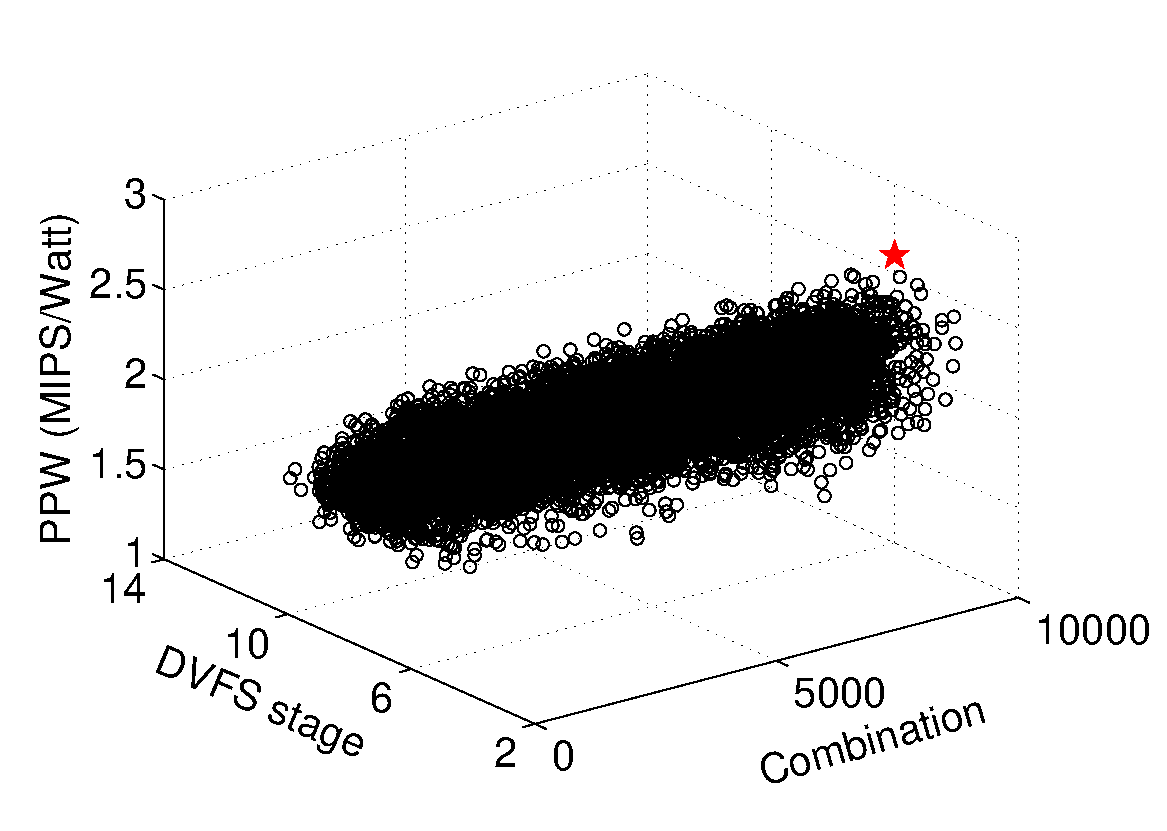
\includegraphics[width=1\linewidth]{fig/best_steady.eps}
\caption{Monte-Carlo of a $16$-core system with $8$ active cores, the variables are the active core distribution and the DVFS stage of each core, the random combination number is 1000, the red pentagram stand for the energy efficiency of our computed power budget}
\end{figure}





In addition to the case shown above, we also tested many other systems with different numbe of cores and active cores. The energy efficiency of these cases are shown in Table~\ref{tab:PPW_steady}. For all cases, the energy efficiency of our given power budget is close to the optimal result.





\begin{table}
%  \color{red}
  \caption{Energy efficiency (in MIPS/Watt) and system performance (in MIPS) results comparison of steady state power budgeting. "New" stands for our new power budgeting method, "Random" denotes the averaged result from $10$ random active core distribution with $T_{opt}$ reached for each active core.}
  \label{tab:PPW_perf_steady}
  \centering
  \begin{tabular}{c|c||c|c||c|c}
    \hline
    Core & Active     & \multicolumn{2}{c||}{New} &
                                                     \multicolumn{2}{c} {Random}\\
\cline{3-6}  
\#       &   \#        & PPW & Perf   & PPW  & Perf \\
%\#      &   \#         & (W)        &      &   (W)   &    &  (W)    &    &(W)   &  (W)\\
     \hline
\hline
  \multirow{3}{*}{9} &      2     &       2.8    & 137.1     & 2.8 & 118.0\\ 
             &      4             &      2.6     & 227.4     & 2.6 & 186.6\\
             &      7             &       2.4    & 290.2      & 2.4 & 262.3\\
     \hline
\multirow{3}{*}{16}   &      3    &      2.6     & 130.0    &  2.6 & 101.5\\   
             &      8             &      2.6    & 243.3    & 2.5 & 185.2 \\
             &      13            &      2.3     &  270.6   &  2.3 & 237.9\\
     \hline
 \multirow{3}{*}{25}  &      5    &     2.8   &  131.7    & 2.8 &111.8       \\ 
                &     12          &     2.8   &   232.3  & 2.8  & 175.3    \\
                &     20          &     2.7   &   271.2    & 2.7 & 230.5 \\
     \hline
  \multirow{3}{*}{36}  &     8            &      2.8   & 142.0    &  2.8  &111.0    \\
              &     18            &     2.7         & 228.9   &  2.7  & 169.0 \\
              &     28          &        2.6      &   263.2     &  2.6 & 230.2 \\
     \hline
 \multirow{3}{*}{64}   &     12           &     2.7  & 132.2   &     2.7   & 102.7  \\
              &     32      &      2.8      &     230.7     &    2.8   & 210.2  \\
              &     52        &      2.4       & 245.7       &  2.4   & 215.6   \\
              
 \hline 
 \multirow{3}{*}{100} & 16 & 2.8 &  122.6    &   2.8   &   93.1  \\
                      & 52 & 2.7 &  242.1     &   2.7   &   212.5  \\
                      & 76 & 2.4 &  285.7     &   2.4   &   252.8  \\
\hline
  
\end{tabular}
\end{table}


Next, we test the power budget quality provided by our method. The results are collected in Table~\ref{tab:PPW_perf_steady}. For comparison, we randomly generate $10$ active core distribution for each case, and compute the averaged energy efficiency and averaged performance with the $T_{opt}$ reached for each active core. As the Table~\ref{tab:PPW_perf_steady} shows, our method provides the optimal performance while the energy efficiency is maximized.


\subsection{Energy-efficient power budgeting with optimal performance considering transient effects}

\begin{figure}
\centering
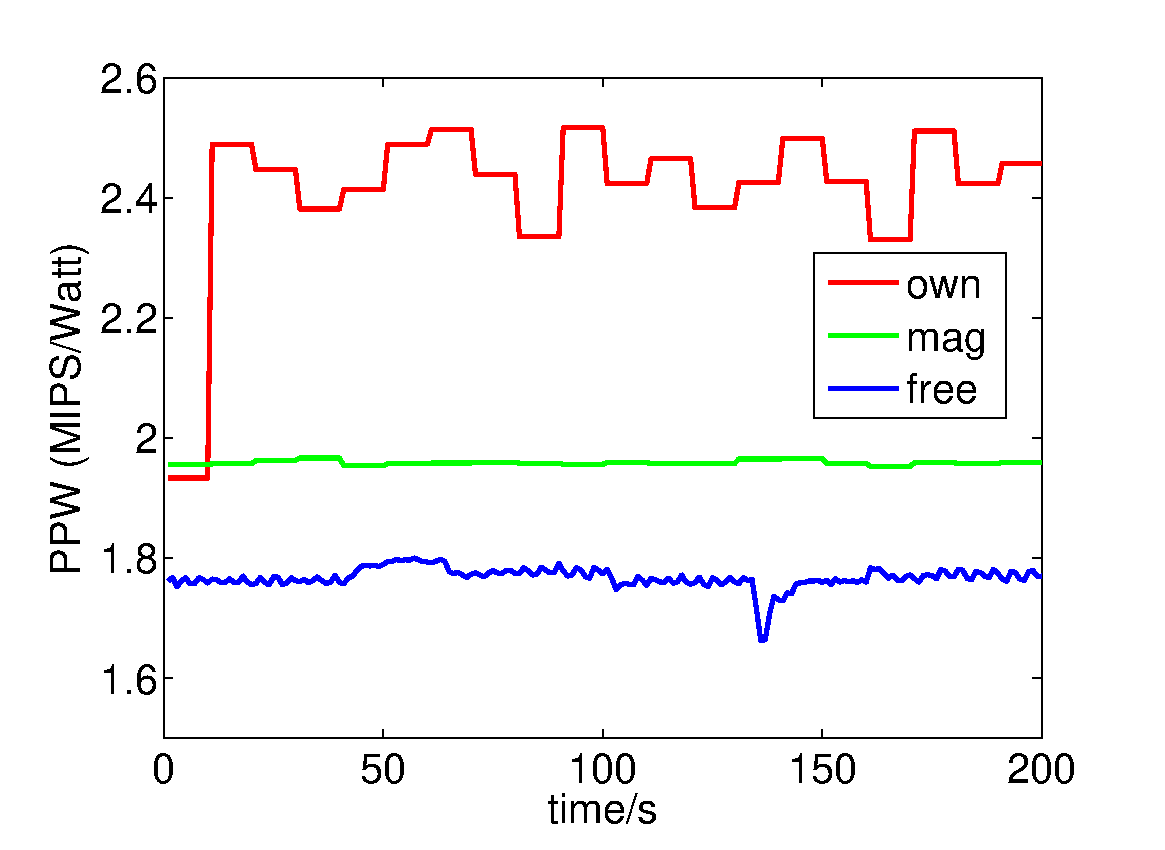
\includegraphics[width=1\linewidth]{fig/PPW.eps}
\caption{PPW}
\end{figure}

\begin{figure}
\centering
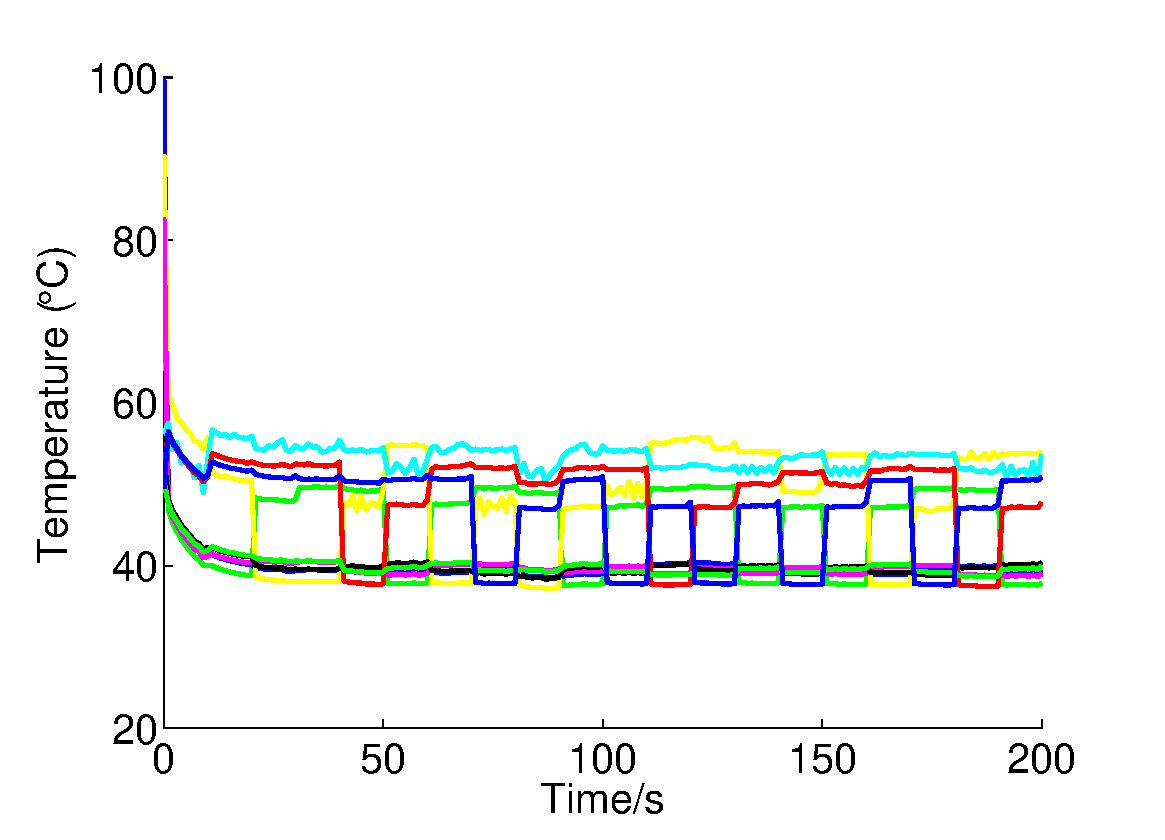
\includegraphics[width=1\linewidth]{fig/tem_own.eps}
\caption{temperature of own}
\end{figure}

\begin{figure}
\centering
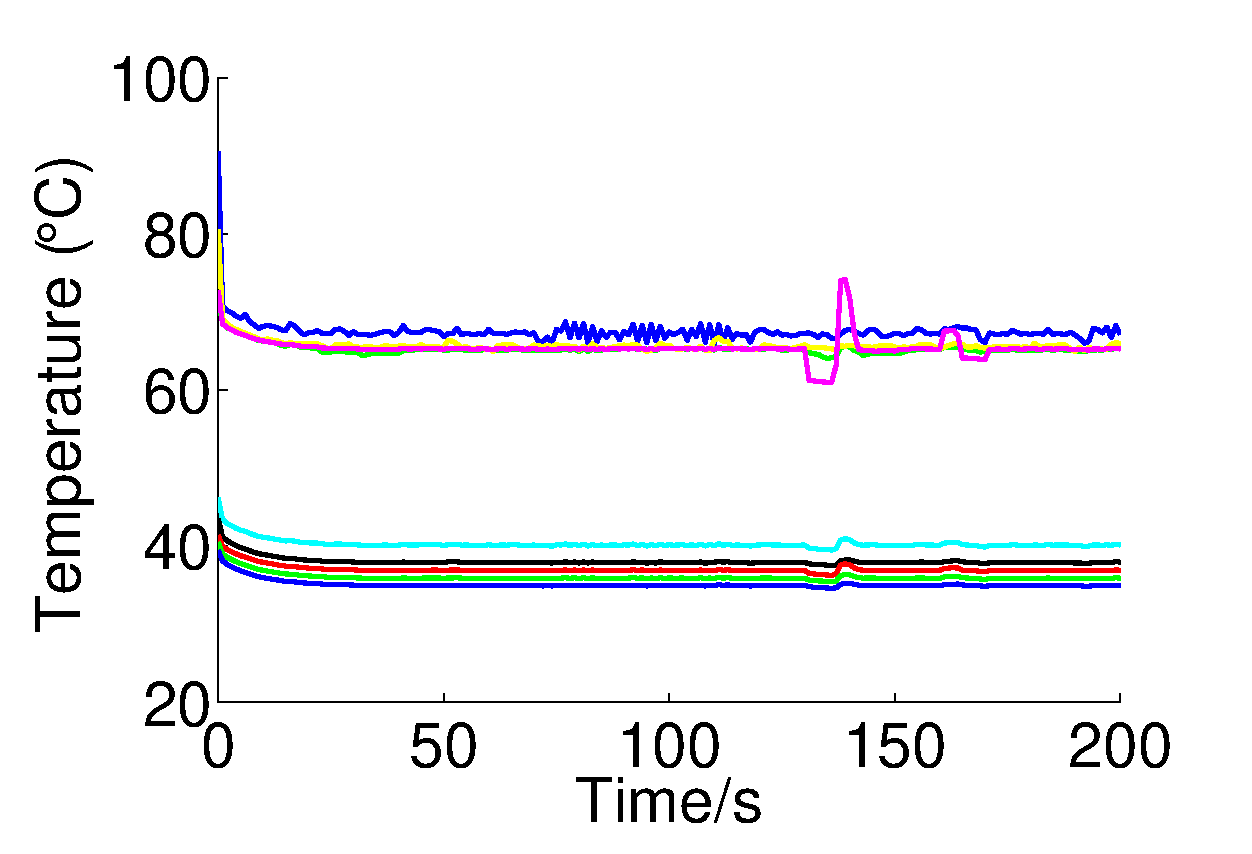
\includegraphics[width=1\linewidth]{fig/tem_mag.eps}
\caption{temperature of mag}
\end{figure}

\begin{figure}
\centering
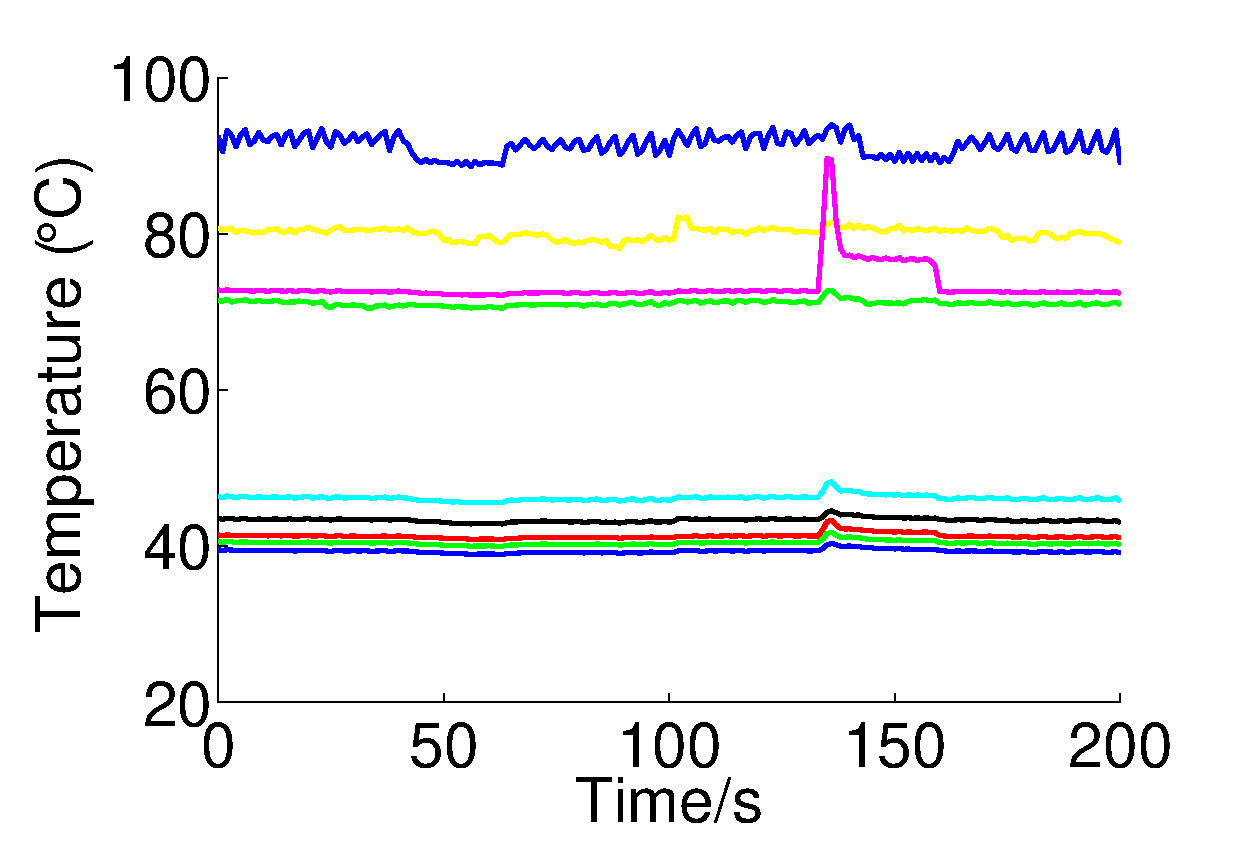
\includegraphics[width=1\linewidth]{fig/tem_free.eps}
\caption{temperature of free}
\end{figure}

\begin{figure}
\centering
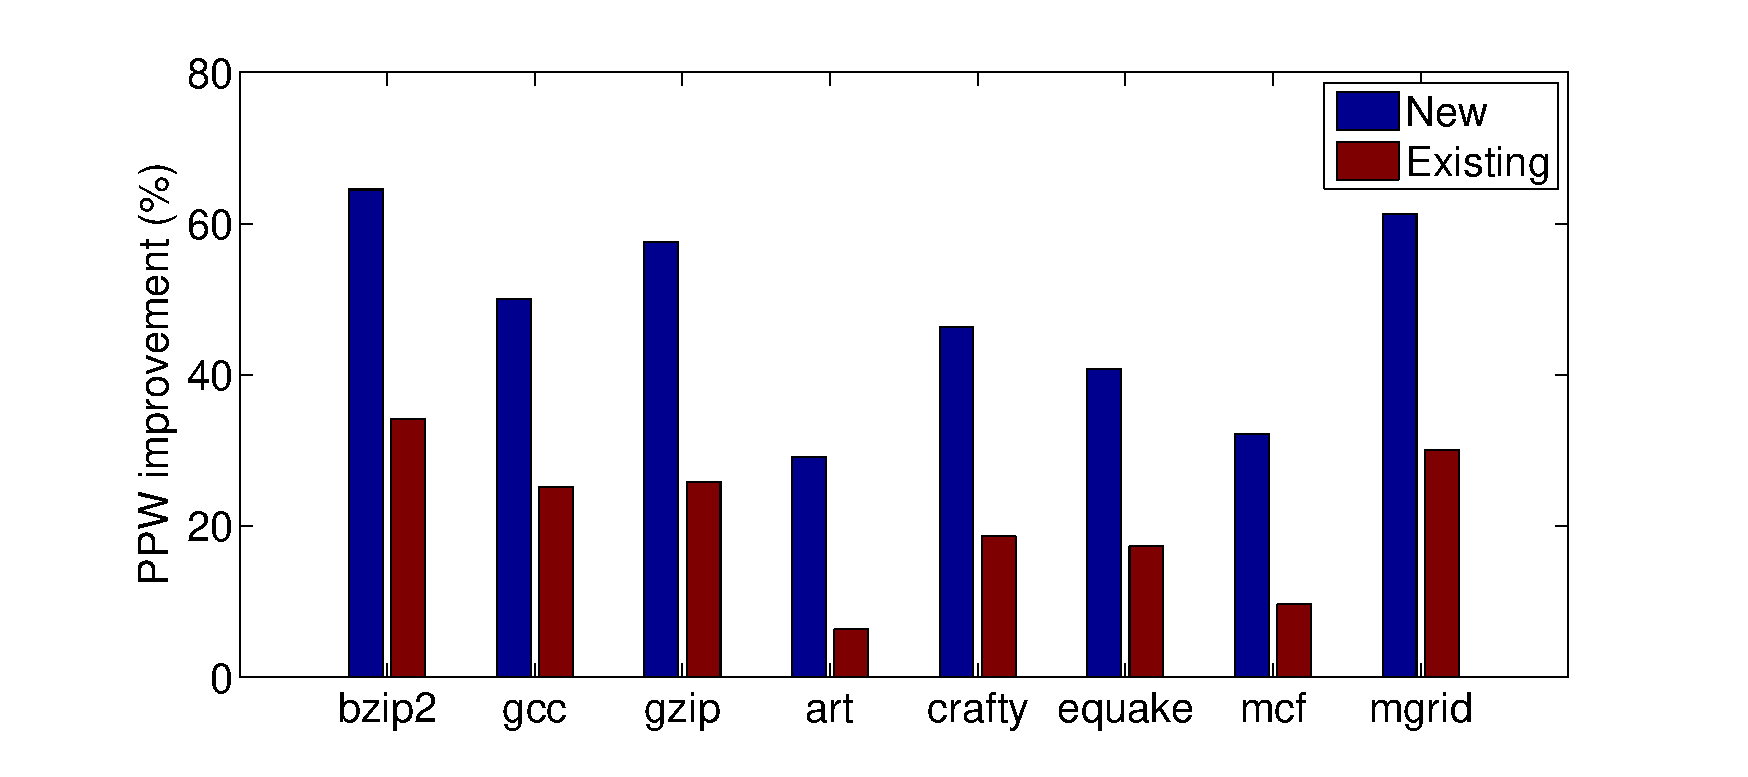
\includegraphics[width=1\linewidth]{fig/transient_ppw.eps}
\caption{ppw improvement comparison}
\end{figure}


Lack one table of dynamic power budgeting's energy efficiency comparison.